oubsection \Sec{rbc} represents `outreach' to the  Computational Fluid Dynamics~(CFD) community,
to give them `some feel' for the basic physical issues at stake, similarly \Sec{cap}  tries
to illustrate the sheer power of the Exascale.  The following subsection~\Sec{alt} discusses approaches that
were raised during Y1 by a range of potential collaborators, and the last subsection~\Sec{pot} elaborates
a potential addition to the \nep \ tasks.

\subsection{SOL and PFC as convection problem}\label{sec:rbc}
\begin{figure}
\centerline{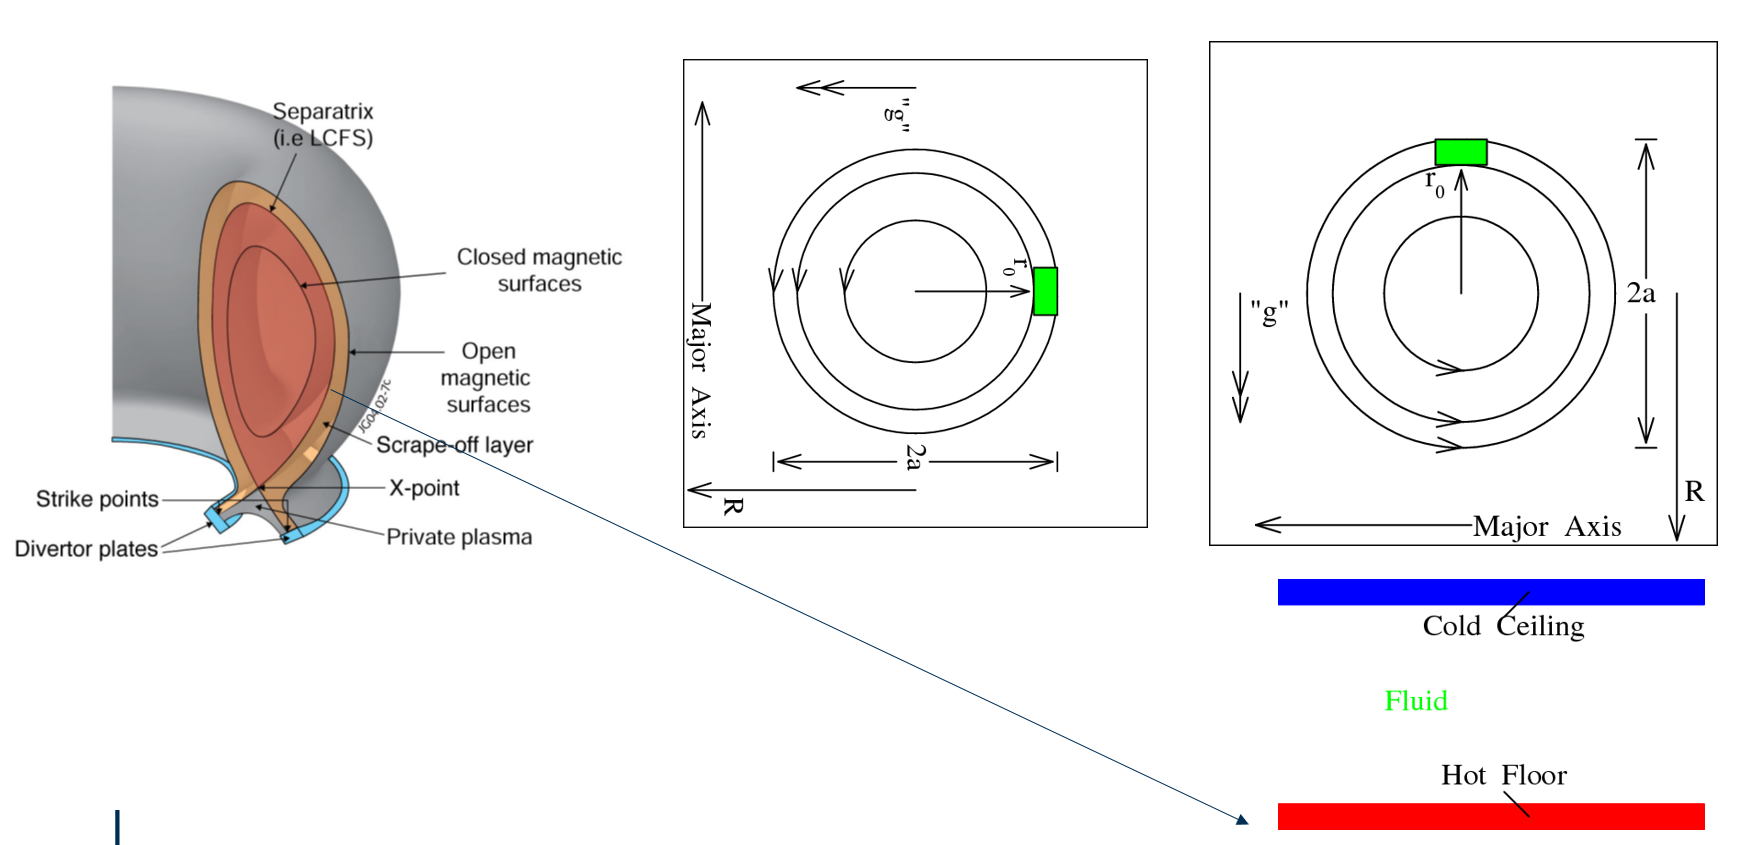
\includegraphics[width=13cm]{../png/rbc}}
\caption{Relationship between the tokamak edge and classical fluid dynamics\label{fig:rbc}.
The plot at far left is courtesy EUROfusion~\tt{eurofusion.org}.}
\end{figure}
To give the specialists in  Computational Fluid Dynamics~(CFD)
a feel for the problem, \Fig{rbc} shows how the outer part of
the midplane (green box) can be approximated as a classical Rayleigh-Benard convection~(RBC) problem,
see the recent work~\cite{Wi19Stab}.
Plasma wants to flow along fieldlines, but there is no escape from the effects of
momentum conservation, and the net result is that plasma experiences an inward
acceleration~$g$. Rotating the picture through $90^o$ so this acceleration looks vertical
makes clearer the relation. The hot central plasma represents a heated floor capable of
driving convection in the SOL.
For RBC, Reynolds numbers and boundary layer thicknesses have been fitted
by Grossmann \& Lohse~\cite{Gr00Scal}. Estimates of the dimensionless
pressure/temperature difference or Rayleigh number~$Ra$ range in the tokamak edge~\cite{Wi19Stab}
plausibly from $10^5-10^{12}$. Assuming a Prandtl number~$Pr\approx 1$,
where $Pr$ is the ratio of viscous to thermal diffusion,
the Reynolds~$Re$ number varies from $Re=10-4\times10^4$. Such values
imply relatively narrow boundary layers, thickness$\propto 1/\sqrt{Re}$
and turbulence for most of the range.


\begin{figure}
\centerline{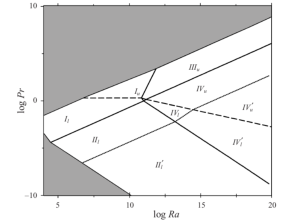
\includegraphics[width=12cm]{../png/Gr00Scal-f2}}
\caption{Ten regimes of RBC depending on the parameters~$Ra$ and $Pr$.
Reproduction of Fig.~2 from ref~\cite{Gr00Scal}. \label{fig:grossmanlohse}}
\end{figure}
\begin{figure}
\centerline{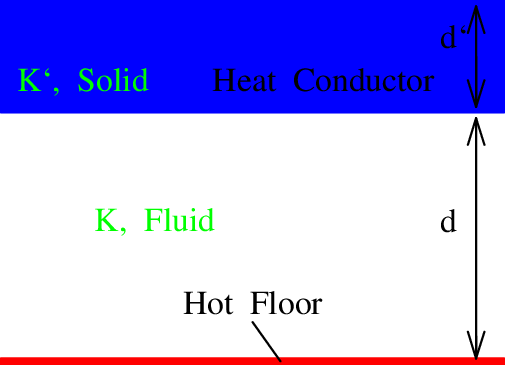
\includegraphics[width=8cm]{../png/RJsl}}
\centerline{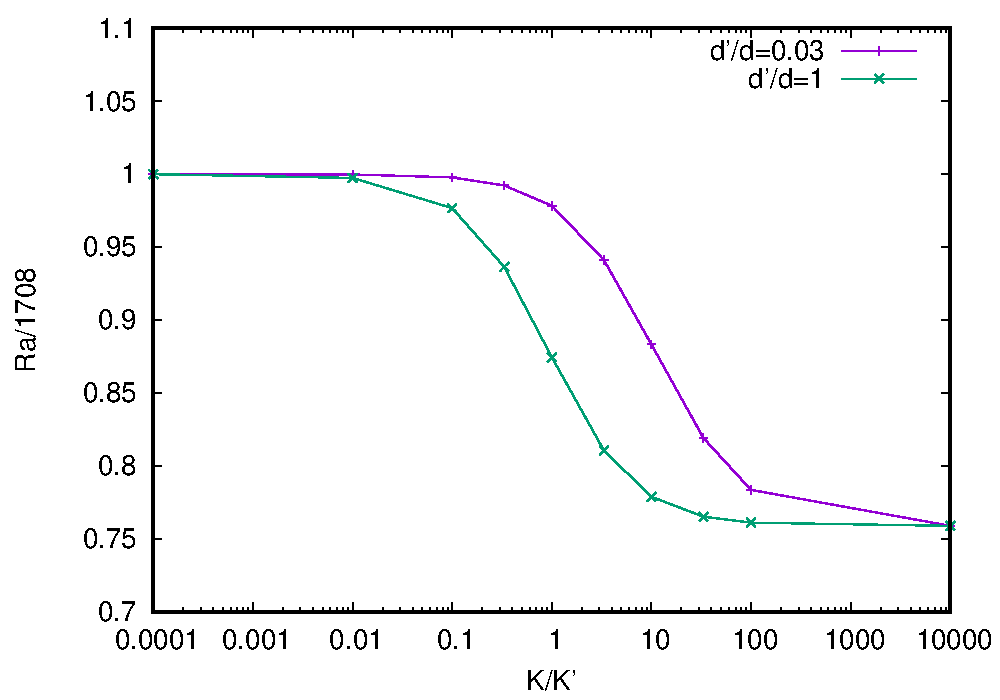
\includegraphics[width=8cm]{../png/rcr2}}
\caption{
Sketch at top of the so-called Rayleigh-Jeffreys problem, where a solid
of thermal conductivity~$K'$ overlies a fluid with thermal conductivity~$K$
Below is plot of normalised critical~$Ra$ as the ratio of conductivities changes.
Data from ref~\cite{Ni68Rayl}. \label{fig:nield}}
\end{figure}
\begin{figure}
\centerline{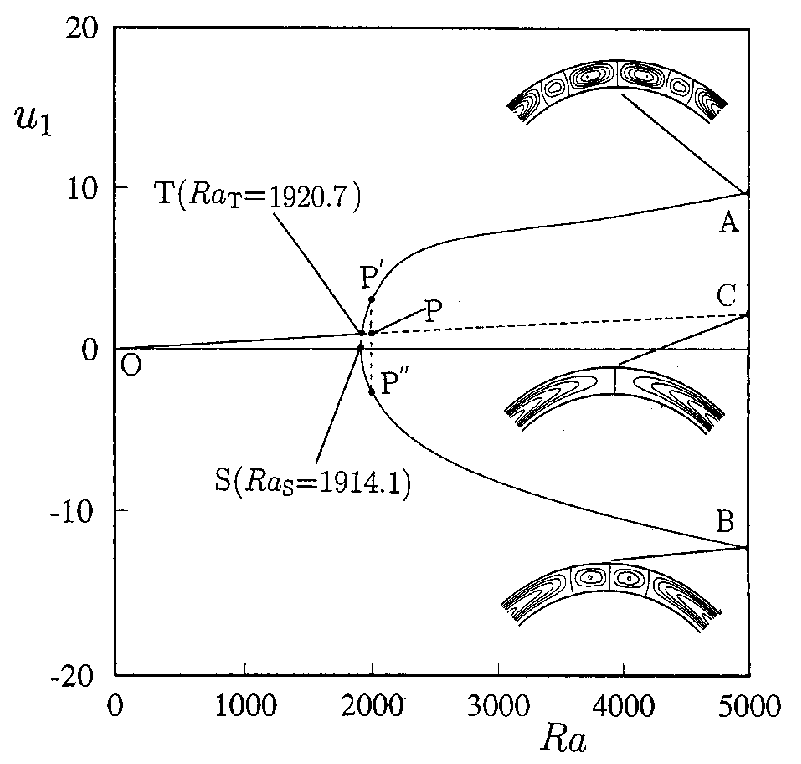
\includegraphics[width=13cm]{../png/Mi01f2c}}
\caption{Amplitude plotted against~$Ra$ at fixed~$Pr$ showing the
interaction between the `double-glazing' solution branch which becomes
unstable at small~$Ra$ and the classical RBC branch which appears beyond $Ra\approx1900$.
Reproduction of Fig.~2 from ref~\cite{Mi01Tran}.  \label{fig:Mi01Tran}}
\end{figure}
It is worth remembering that the Rayleigh-Benard problem, while simple to pose, is hard to
understand fully, and sensitive to details of both boundary conditions and geometry.
For example, 
\begin{enumerate}
\item for the scaling of dimensionless heat flux~$Nu$ with convection, there are ten regimes of RBC depending on the temperature difference measured by Rayleigh number~$Ra$
and Prandtl number $Pr=Ku/K$, see \Fig{grossmanlohse}. The scaling law exponents $\gamma_1$, $\gamma_2$ which are
defined so that $Nu \propto Ra^{\gamma_1} Pr^{\gamma_2}$ range over $1/4 < \gamma_1 < 4/7$ and
$-5/6 < \gamma_2 < 1/8$.
\item  there is an approx.\ 70\,\% reduction in heat flux if the boundary condition on the
flow is changed from free-slip to stagnation. This follows because the critical~$Ra$,
 $Ra_C\approx657$ increases to $Ra_C\approx1708$~\cite{chandrasekhar},
and from assuming that heat flux~$Nu\propto (Ra-Ra_C)^{1/2}$.
\item there is an approx.\ 10\,\% increase in~$Nu$ possible due to a change outside the fluid region, 
namely the replacement of perfectly conducting boundaries by poor insulators, see \Fig{nield},
understood from the fact that a poorly conducting boundary constrains the convection less.
\item  in a heated annulus, which \Fig{rbc} suggests is a more accurate model of the edge,
there is a complex bifurcation structure possible, see \Fig{Mi01Tran}.
\item  there are indications that Fourier spectral (and probably other numerical) schemes converge
non-monotonically as spatial resolution increases, eg.\ the reduction of RBC to the Lorenz equations~\cite{Lo63Dete}
does not permit smaller-scale instability of thermal boundary layers because it represents them too crudely.
However, more detailed, but unresolved models of these layers may exhibit time-dependence 
when the full solution with thinner layers does not, because layers of thickness~$d$ are destabilised
by a term$\propto d^3$.
\end{enumerate}



\subsection{Capabilities of the Exascale}\label{sec:cap}
In the tokamak edge, following~\cite{Wi19Stab}, 
suppose plasma number density $n \approx 10^{18}$\, m$^{-3}$. Order of magnitude
dimensions are $L\approx0.1$\,m for SOL thickness, reactor minor and major radii
say $a=3$\,m and $R_0=10$\,m, so volume of SOL $\approx 4 \pi^2 a R_0 L \approx 100$\,m$^3$.
Hence total number of electrons $\approx 10^{20}$.

Shortest timescale is inverse $e B/m_e$, the electron cyclotron frequency, where
$e/m_e = 1.76 \times 10^{11}$\,C kg$^{-1}$, and $B\approx 10$\,T, so $\tau_{Be}\approx 10^{-12}$\,s.
Hence number of particle-steps to evolve $1$\,s of physical time is  $10^{20+12+1}$,
and assuming $1000$\,flop per update, need $10^{36}$\, flops.
So to complete in $1$\,s on Exascale machine, only allowed to sample $1$~particle-step in $10^{18}$.
(Unlikely to be adequate because of electrostatic and other effects.)

Suppose fluid instead, ie.\ representing electron distribution by first~$3$ moments.
Electron temperature~$T_e \approx 10$\,eV,
thermal speed $V_{Te}\approx 10^6$\,m s$^{-1}$. Sample SOL at uniform $1$\,mm interval,
number of sample-points $\approx 10^{11}$, timestep for explicit scheme $\approx 0.1 \times (10^{-3} /10^6)$
so number of sample-point updates is $10^{11+10}$, assume  $1000$\,flop each update, need $10^{24}$\, flops.

Another way, suppose numerical problem is $D$-dimensional, need $1000$\,flop each sample update
and allowed $N_D$~samples per spatial dimension and $N_D^2$ in time. Then to update in $1$\,s, have
$N_D^{D+2} \approx 10^{15}$. Thus  if $D=3$, $N_3 \approx 1\,000$, and $N_5 \approx 100$.
\emph{Accuracy controlled, unstructured, implicit fluid models should be possible.}

Similarly, estimates of the maximum frequency at which neutral atom particle-steps can be sampled,
assuming $n_0=n$ and $T_0 =T_e$, indicates that useful results may be obtained from the particle approach.
Moreover, repeating the above calculation for electrons but considering that only plasma ions have
to be simulated on a drift type timescale$\approx L/V_{Ti}$,
$V_{Ti}\approx 3 \times 10^4$\,m s$^{-1}$, gives much more encouraging results.

\subsection{Alternative Approaches}\label{sec:alt}
The 2nd Edition of the Encyclopedia of Computational Mechanics~\cite{encyclcompmech}
contains up-to-descriptions of a large range of techniques for solving problems in
elasticity theory and/or fluid dynamics. It is noteworthy that there is an almost complete
absence of UK addresses among the contributors, reflecting a US and European bias in the editorial
board. Even though the Encyclopedia is demonstrably not comprehensive, notably when it comes to
what the editors would probably regard as more speculative schemes, if anyone in the requirements
capture exercise had admitted to reading through ref~\cite{encyclcompmech},
considerable attention would have been paid to their views. 

\emph{Note that citations and scoring in this
section reflect an idiosyncratic reading of a very wide field 
and are subject to revision.}

In the event, during the requirements capture exercise, several other possible approaches were
mooted in addition
to spectral/hp element~(SHP), which has Galerkin, discontinuous Galerkin and semi-Lagrangian
formulations~\cite{karniadakissherwin}.
It was commented that it would be relatively straightforward to adapt the SHP libraries for IGA,
see below.
Discounting special pleading, those felt worthy of mentioning were
\begin{enumerate}
\item Discontinuous Galerkin with usual (polynomial) finite element bases~(DG)~\cite{hesthavenwarburton}
\item Isogeometric finite element bases~(IGA)~\cite{Hu18Math} % TJR Hughes in Wiley Vol.2
\item Lattice Boltzmann~(LB)~\cite{Ro19Univ}
\item Smoothed Particle Hydrodynamics~(SPH)~\cite{violeau}
\item Dedalus software~\cite{Bu19Deda}
\end{enumerate}
The AMR work of Nikiforakis and coworkers, eg.~\cite{Go18dime} may be regarded as special pleading, but since it also has
implications for geometry representation, it is discussed in the Milestone Report~\cite{y1re211}.
In addition the following are tabulated in Table~\ref{tab:assess}.
\begin{enumerate}
\item Sparse grids~\cite{He03Adap,Bu04Spar}
\item Radial basis functions~(RBFs)~\cite{fornbergflyer}
\item Arbitrary Lagrangian-Eulerian~(ALE)~\cite{Do18Arbi}
\end{enumerate}
Proponents of other approaches should be prepared to score them also.

\begin{table}[h]\label{tab:assess}
\begin{center}
\caption{Preliminary scoring of plausible schemes for \nep\ use. At the present date, the ability to represent geometry
and the availability of UK skills would seem most important.}
\begin{tabular}{|p{2cm}|p{2.2cm}|p{1.8cm}|p{2.6cm}|p{1.8cm}|p{1.8cm}|}
\hline
Approach & Maturity~(TRL) & Geometry & (Exa)Scalability & Efficiency & UKRI skills \\
\hline
 SHP & $5$ & $5$ & $5$ & $5$ & $5$ \\
 DG & $5$ & $5$ & $5$ & $4.5$ & $3$ \\
 AMR & $4$ & $4$ & $5$ & $4.5$ & $5$ \\
 IGA & $3$ & $2$ & $3$ & $5$ & $1$ \\
 LB & $5$ & $2$ & $5$ & $3$ & $3$ \\
 SPH & $5$ & $4$ & $3$ & $1$ & $3$ \\
 Dedalus & $5$ & $4$ & $3$ & $4$ & $3$ \\
 Sparse & $3$ & $2$ & $2$ & $5$ & $1$ \\
 RBF & $3$ & $3$ & $3$ & $5$ & $1$ \\
 ALE & $4$ & $4$ & $5$ & $5$ & $1$ \\
\hline
\end{tabular}
\end{center}
\end{table}


Note that the scores correspond to
\begin{enumerate}
\item TRLs for Software
\begin{itemize}
\item[1] Scheme properly defined
\item[2] Scheme analysed
\item[3] Software for single user
\item[4] Software for multiple users
\item[5] Software for multiple users and usages
\end{itemize}
\item Complexity of geometry modelled
\begin{itemize}
\item[1] Slab geometry
\item[2] Simple 2-D or 3-D geometry
\item[3] Complex 2-D geometry
\item[4] Complex 3-D geometry
\item[5] Complex 3-D geometry to high order
\end{itemize}
\item Scalability
\begin{itemize}
\item[1] Poor theoretical and demonstrated
\item[2] Good theoretical (Cluster)
\item[3] Good demonstrated (Cluster)
\item[4] Very Good theoretical (at Petascale)
\item[5] Very Good demonstrated (at Petascale)
\end{itemize}
\item Efficiency
\begin{itemize}
\item[1] Scales as $1/\sqrt{N}$
\item[2] Scales as $1/N$
\item[3] Scales as $1/N^{k}$, fixed $k>1$
\item[4] Spectrally accurate
\item[5] Spectrally accurate, grid refinable or better than spectral
\end{itemize}
\item UKRI skills available
\begin{itemize}
\item[1] No evidence
\item[2] Ability to use code
\item[3] Ability to use code and understand limitations
\item[4] Demonstrated ability to modify code
\item[5] Significant part of code written in UK
\end{itemize}
\end{enumerate}


There are also items which involve other mathematical reformulation of the problem, notably
\begin{itemize}
\item Asymptotic-Preserving Methods~(APM)~\cite{De17Asym}  %degond deluzet
\item Variational (Lagrangian and Hamiltonian) formulations, see presentations at INI GCS meeting
\item Lie derivative approaches~\cite{Ar19Chal-ppt}
\end{itemize}
These are candidates for the \exc \ Cross-Cutting Programme.


\subsection{Potential Additions to \nep }\label{sec:pot}

\subsubsection{Adjoint or `dual' approach}\label{sec:dual}
The adjoint approach to sensitivity analysis exploits the fact that
the sensitivity of only one or perhaps a small number of quantities
such as~$Q$, each a linear combination of the ~$N_i$ is needed.
The technique is best illustrated~\cite{Gi00Intr} by a simple, linear example.

Imagine that the problem being solved is the
(`primal') set of linear equations for unknown~${\bf x}$,
namely $A {\bf x}= {\bf b}$ to find one
quantity (the 'objective function')~${\bf g}^T {\bf x}$, where the
vectors ${\bf b}$ and~${\bf g}$ are given.
It happens that the same result may be achieved by solving instead
the (`dual') equation set~$A^T {\bf v}= {\bf g}$ and
forming ${\bf v}^T {\bf b}$.
This may be demonstrated by one line of matrix-vector algebra:
\begin{equation} \label{eq:dualequiv}
{\bf v}^T {\bf b} = {\bf v}^T A {\bf x} = (A^T {\bf v})^T {\bf x} = {\bf g}^T {\bf x}
\end{equation}
It should be apparent that if the objective function is to
be evaluated for $K$~different vectors~${\bf b}$, but only one~${\bf g}$,
only one dual solution is needed,  not $K$~primal solutions.
Provided one dual solution is not significantly more costly than one primal one, a
significant saving may be realised.

The main tension arises when the model is not self-adjoint, in that
the dual problem is then different from the one that the physicist would like to
understand. This can be an additional reason for preferring a variational approach.

